\documentclass{article}
\usepackage[margin=1in]{geometry}
\usepackage{graphicx}
\usepackage{hyperref}
\usepackage{natbib}
\usepackage{soul}
\bibliographystyle{apalike}
\usepackage{amsmath}

\title{Supplementary Material \\ \large{Fish from the Sky: A Novel Framework for Capturing and Quantifying Aquatic Life via Airborne eDNA}}

\author{Yin Cheong Aden Ip$^1$\textbf{*} \and
Gledis Guri$^1$\textbf{*} \and
Elizabeth Andruszkiewicz Allan$^1$ \and
Ryan P. Kelly$^1$}

\date{\today}

\begin{document}

\maketitle

%\section*{}

\begin{center}
\begin{tabular}{ll}
1 & School of Marine and Environmental Affairs, University of Washington, Seattle, Washington, USA \\
\hline
\textbf{*} & shared first authorship\\
&\\
& corresponding author \textbf{adenip@uw.edu}
\end{tabular}
\end{center}

\clearpage
\begin{figure}[tbhp] 
\centering
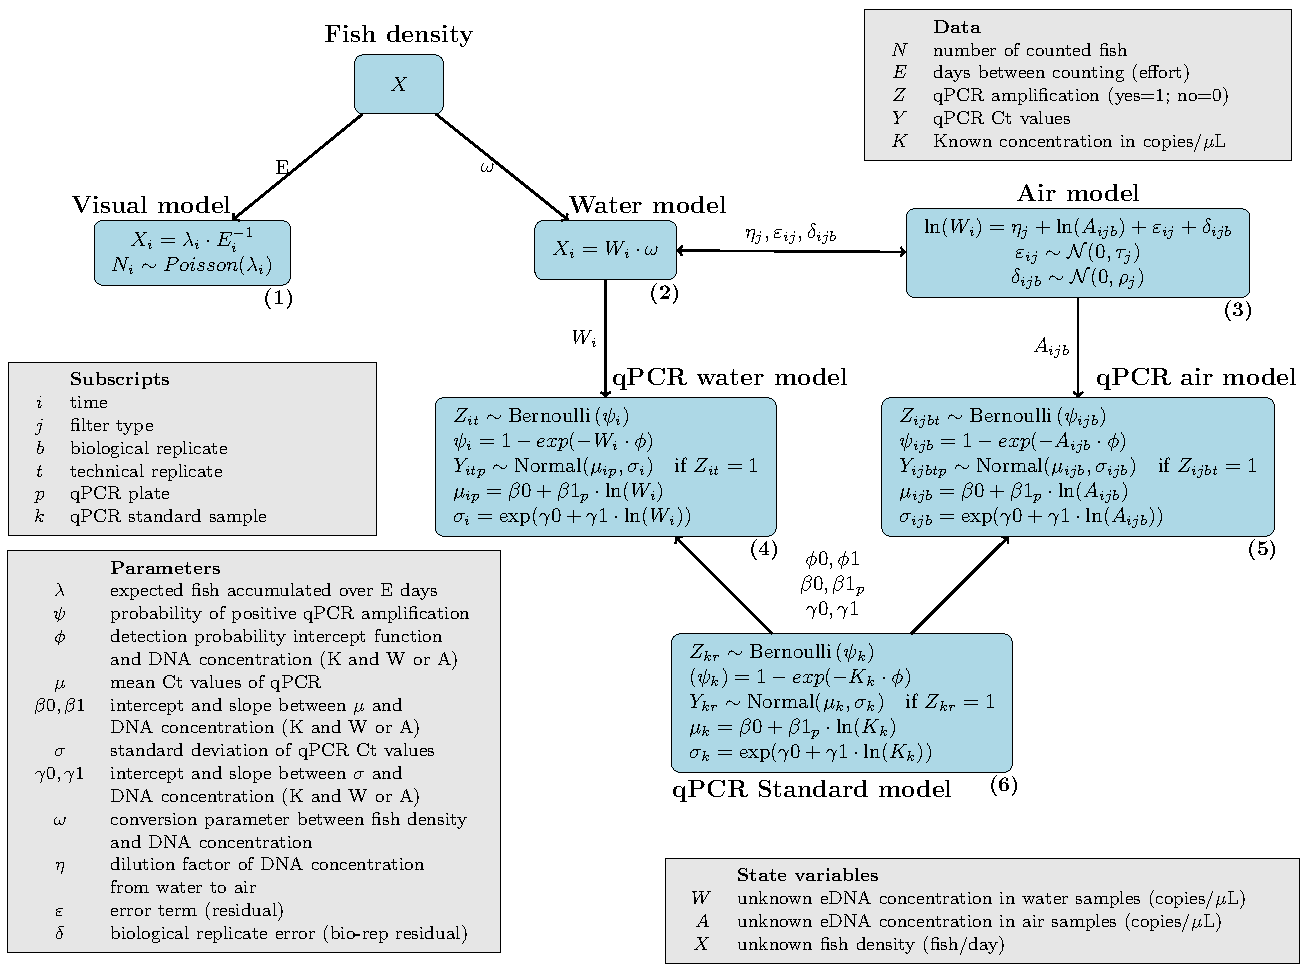
\includegraphics[width=16.5cm]{Plots/DAG.pdf}  
\caption{DAG of joint Bayesian model for estimating the eDNA concentration of Air}
\label{fig:DAG}
\end{figure}


\clearpage
\begin{figure}[tbhp] 
\centering
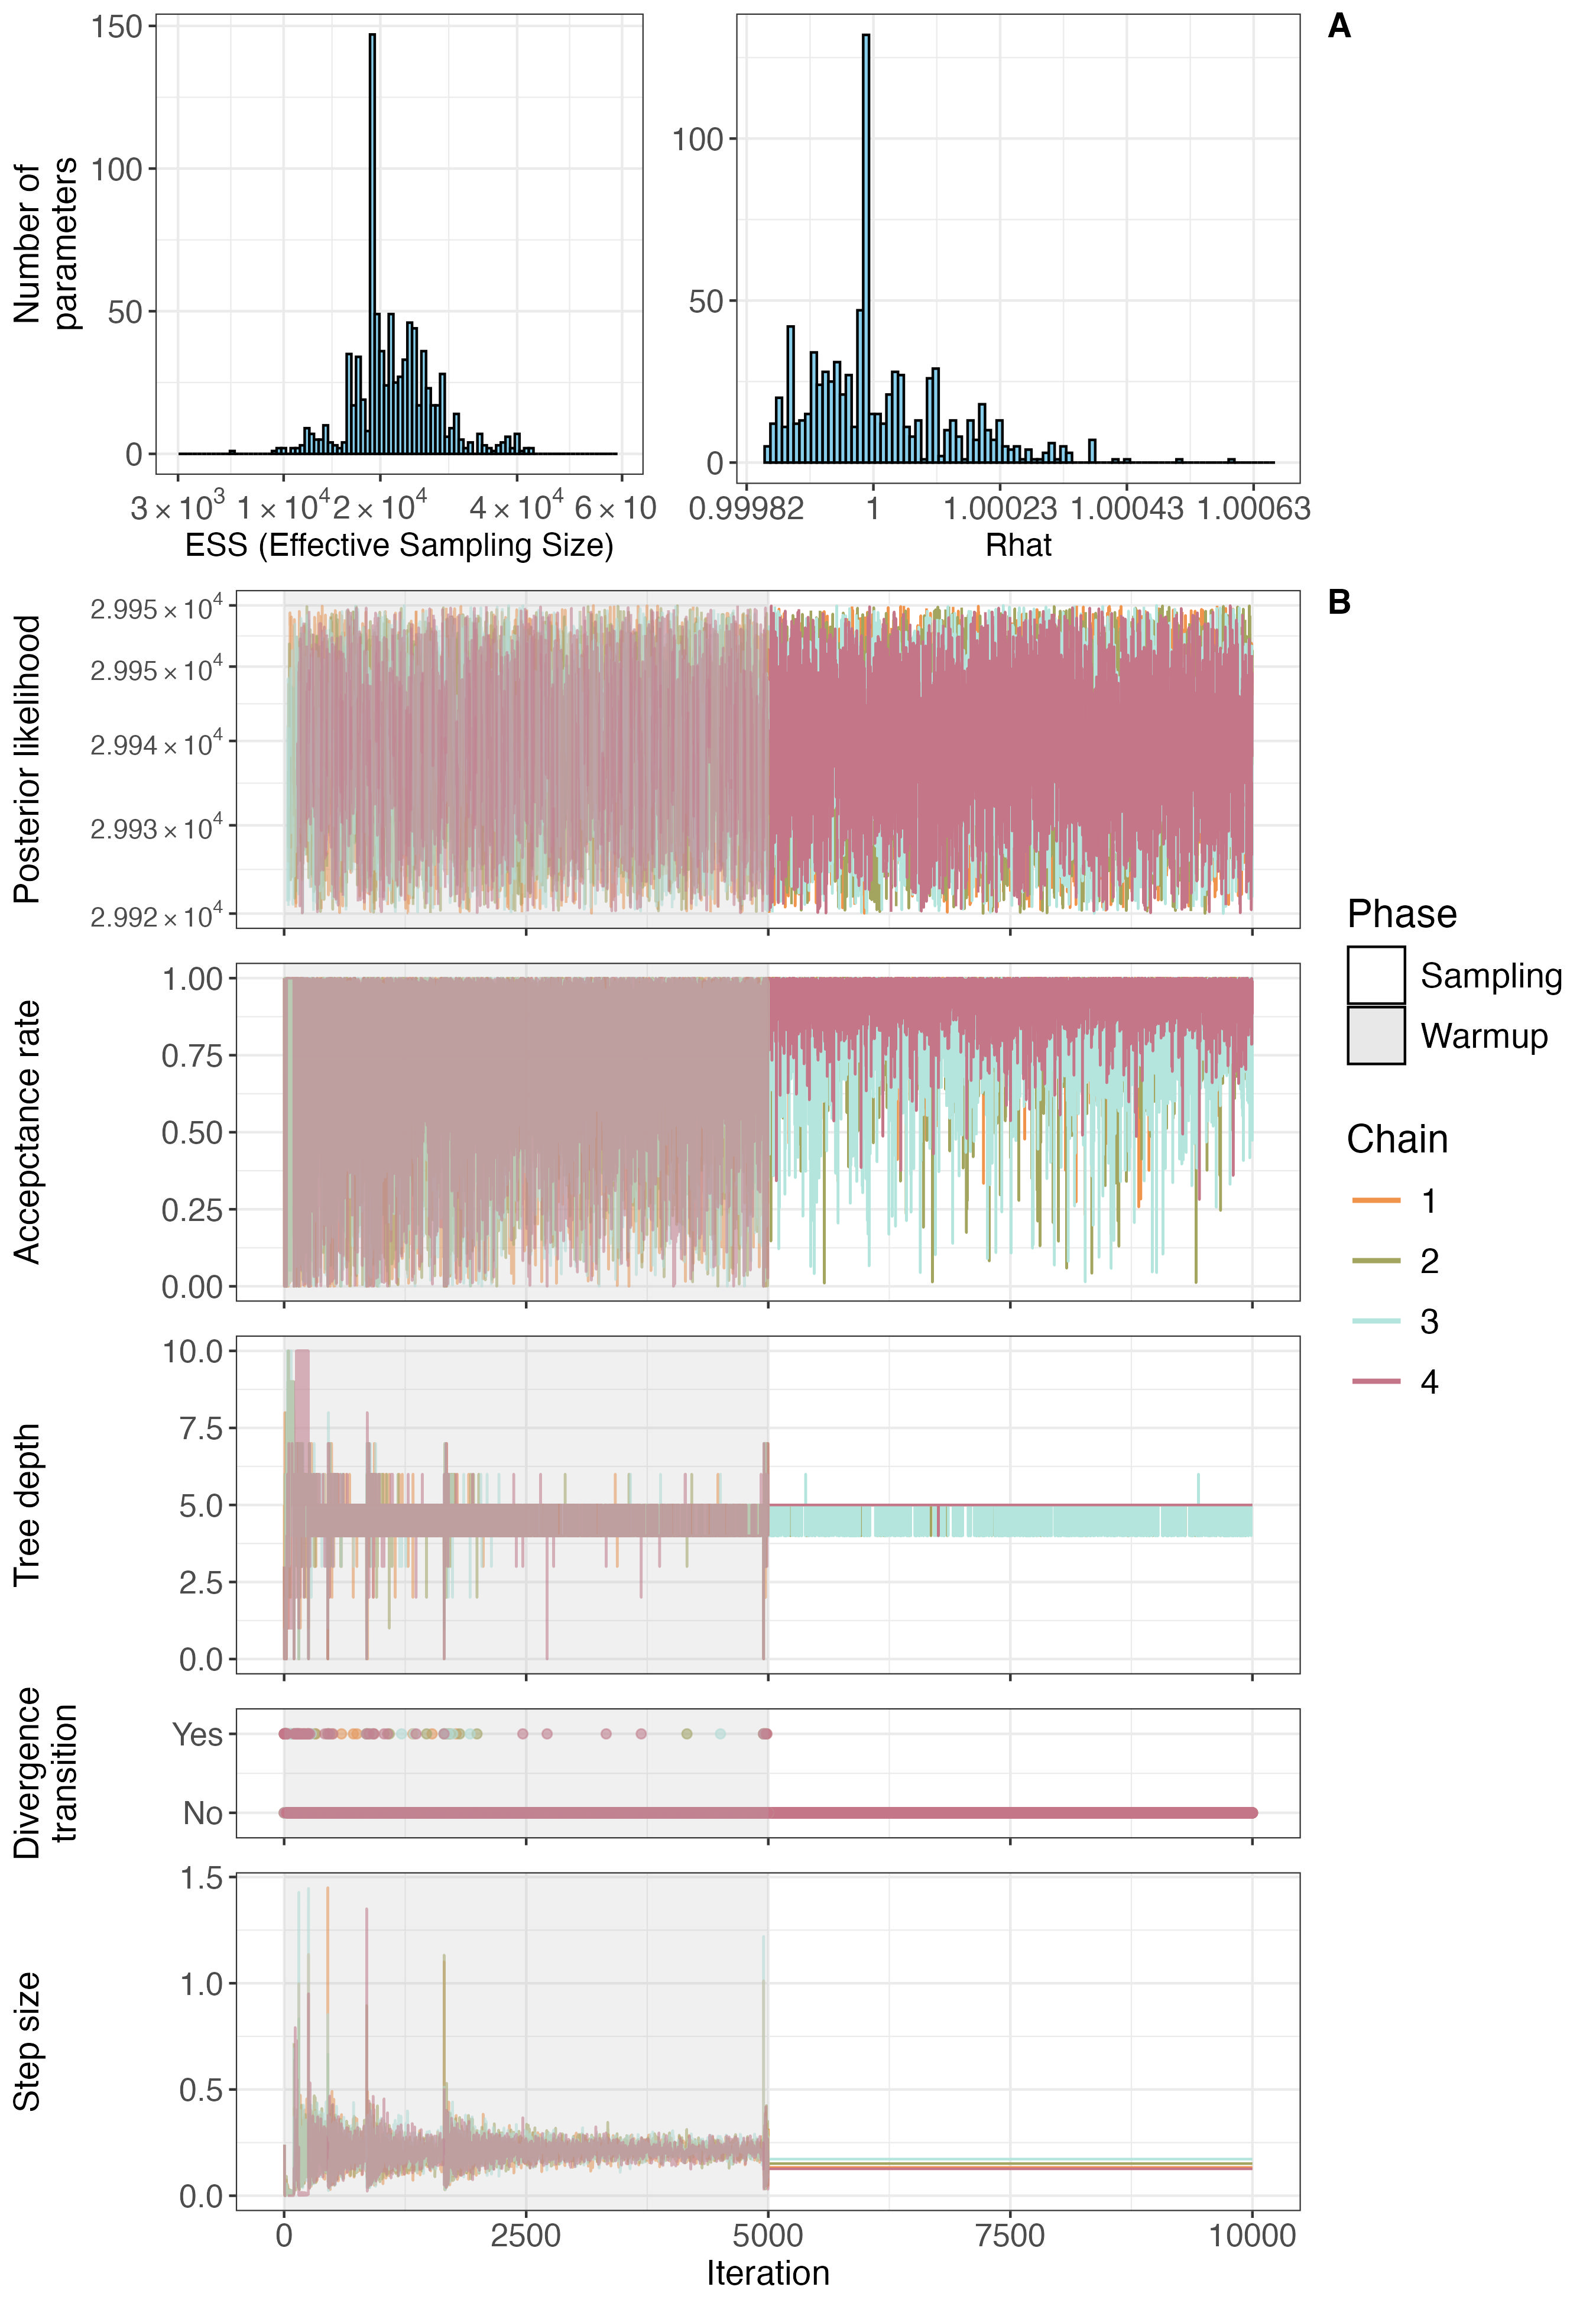
\includegraphics[width=15.2cm]{Plots/Diagnostic_Fig_1.jpg}  
\caption{Model diagnostics}
\label{fig:diagnostics}
\end{figure}

\clearpage
\begin{figure}[tbhp] 
\centering
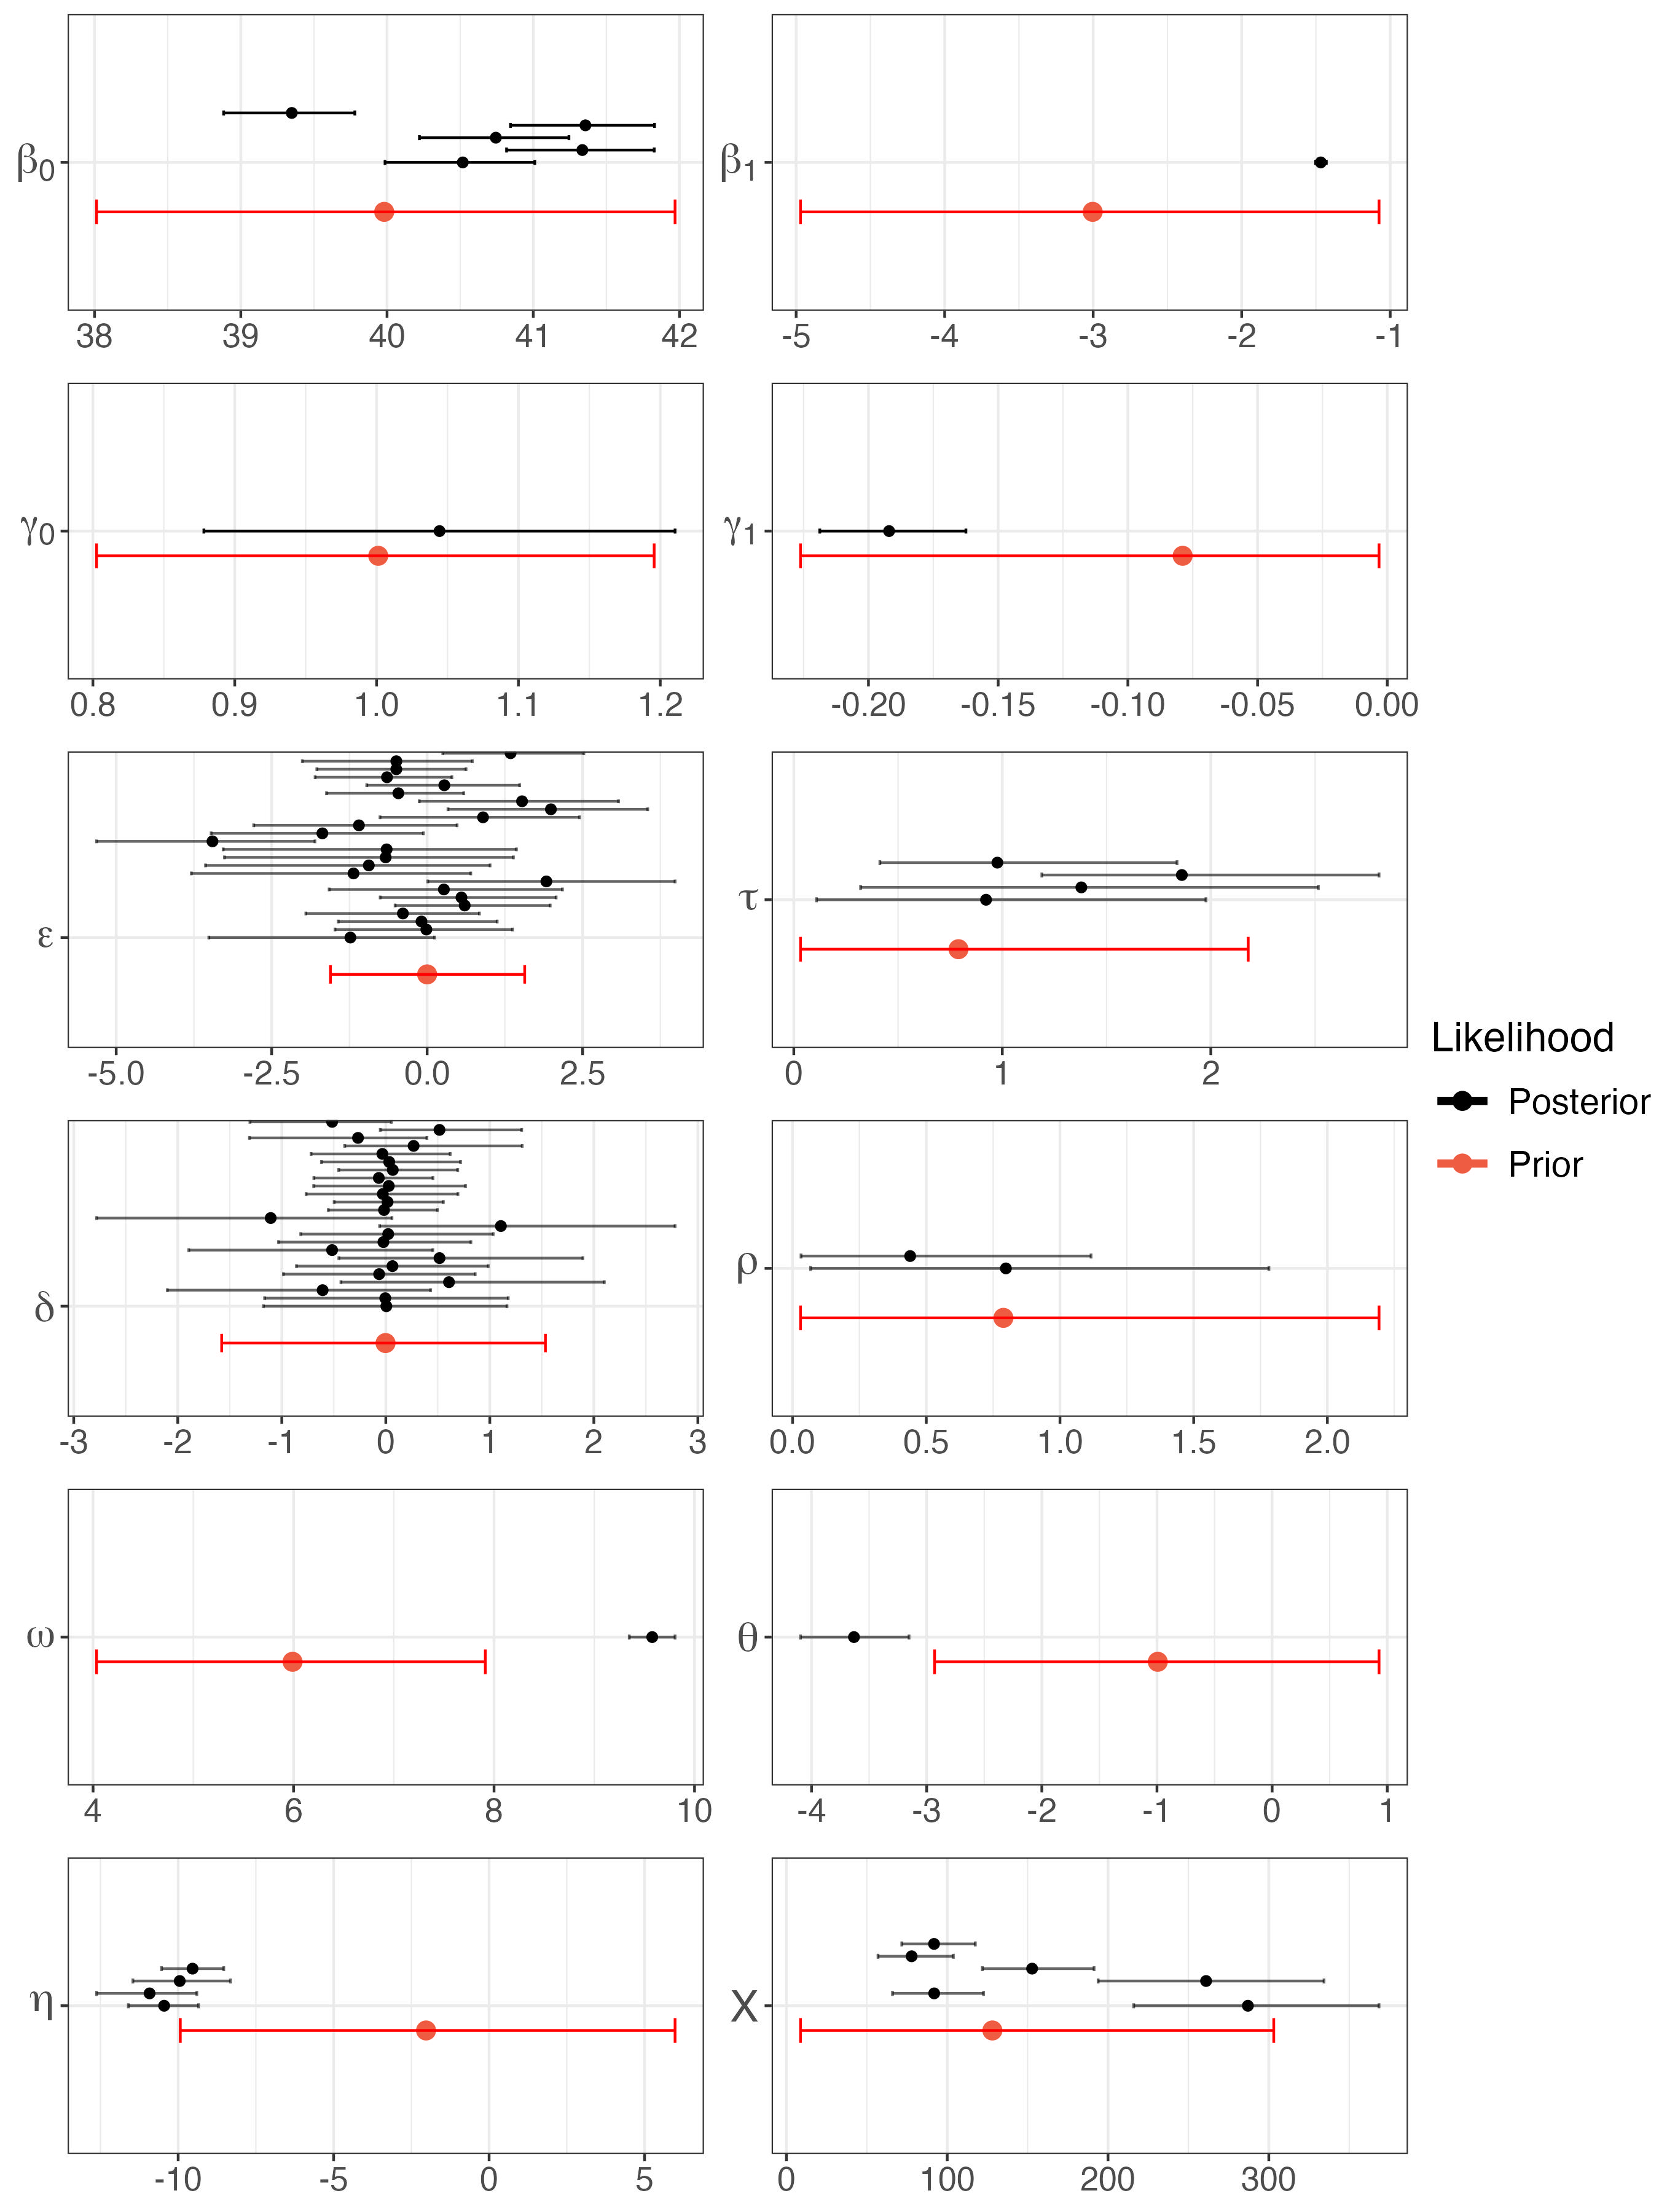
\includegraphics[width=16.5cm]{Plots/Diagnostic_Fig_2.jpg}  
\caption{Prior sensitivity analysis}
\label{fig:prior_sens}
\end{figure}


\clearpage
\begin{table}
    \centering
    \begin{tabular}{lll}
         & \textbf{Description} & \textbf{Prior} \\
&Data & \\
\hline
$N$ & number of fish counted & - \\
$E$ & elapsed days between counting & - \\
$Z$ & qPCR amplification (yes=1; no=0) & - \\
$Y$ & qPCR cycle threshold (Ct) & - \\
$K$ & known DNA concentration (qPCR standards) & - \\

&&\\
&State processes&\\
\hline
$X$ & unknown fish density in (fish $\cdot$ day$^{-1}$) & $\Gamma(10,1)$ \\
$W$ & unknown DNA concentration in water in (copies/L) & - \\
$A$ & unknown DNA concentration in air in (copies/day/cm$^2$) & - \\
&&\\

&Transformed parameters&\\
\hline
$\lambda$& expected fish accumulated over E days & - \\
$\psi$& probability of positive qPCR amplification & - \\
$\mu$& mean Ct values of qPCR & - \\
$\sigma$& standard deviation of qPCR Ct values & - \\
&&\\

&Parameters&\\
\hline
$\omega$& conversion parameter between fish density
and DNA concentration & $\mathcal{N}(0,1)$\\
$\eta$& dilution factor of DNA concentration
from water to air & $\mathcal{N}(0,5)$\\
$\varepsilon$& time ($i$) specific error term (residual) & $\mathcal{N}(0,\tau)$\\
$\tau$& standard deviation of residuals & $\mathcal{TN}(0,1;0, +\infty)$\\
$\delta$& biological replicate error term (residual) & $\mathcal{N}(0,\rho)$\\
$\rho$& standard deviation of biological replicate error & $\mathcal{TN}(0,1;0, +\infty)$\\
$\phi$& intercept of the qPCR probability of detection ($\psi$) relationship &$\mathcal{N}(-1,1)$\\
& and eDNA concentration ($K$, $W$, and $A$) \\
$\beta0$& intercept of the linear relation between the mean Ct values ($\mu$)&$\mathcal{N}(40,1)$\\
&and eDNA concentration ($K$, $W$, and $A$) & \\
$\beta1$& slope of the linear relation between the mean Ct values ($\mu$) and &$\mathcal{N}(-3,1)$\\
&eDNA concentration ($K$, $W$, and $A$)) & \\
$\gamma0$& intercept of the linear relation between the standard deviation&$\mathcal{N}(1,0.1)$\\
&of Ct values ($\sigma$) and eDNA concentration ($K$, $W$, and $A$) & \\
$\gamma1$& intercept of the linear relation between the standard deviation &$\mathcal{N}(0,0.1)$\\
&of Ct values ($\sigma$) and eDNA concentration ($K$, $W$, and $A$) & \\
&&\\
&Index&\\
\hline
$i$& time (days) & -\\
$j$& filter type & -\\
$b$& biological sample replicate & -\\
$p$& qPCR plate & -\\
$k$& qPCR standard sample & -\\


    \end{tabular}
    \caption{Data, state processes, parameters, transformed parameters, and subscripts employed in the joint Bayesian model and their prior distributions}
    \label{tab:priortable}
\end{table}
\clearpage
\bibliography{Bib.bib}
\end{document}

